%%%%%%%%%%%%%%%%%%%%%%%%%%%%%%%%%%%%%%%%%
% a0poster Portrait Poster
% LaTeX Template
% Version 1.0 (22/06/13)
%
% The a0poster class was created by:
% Gerlinde Kettl and Matthias Weiser (tex@kettl.de)
% 
% This template has been downloaded from:
% http://www.LaTeXTemplates.com
%
% License:
% CC BY-NC-SA 3.0 (http://creativecommons.org/licenses/by-nc-sa/3.0/)
%
%%%%%%%%%%%%%%%%%%%%%%%%%%%%%%%%%%%%%%%%%

%----------------------------------------------------------------------------------------
%	PACKAGES AND OTHER DOCUMENT CONFIGURATIONS
%----------------------------------------------------------------------------------------

\documentclass[a0,portrait]{a0poster}

\usepackage{multicol} % This is so we can have multiple columns of text side-by-side
\columnsep=100pt % This is the amount of white space between the columns in the poster
\columnseprule=3pt % This is the thickness of the black line between the columns in the poster

\usepackage[svgnames]{xcolor} % Specify colors by their 'svgnames', for a full list of all colors available see here: http://www.latextemplates.com/svgnames-colors

\usepackage{times} % Use the times font
%\usepackage{palatino} % Uncomment to use the Palatino font

\usepackage{graphicx} % Required for including images
\graphicspath{{figures/}} % Location of the graphics files

\usepackage{caption}
%\usepackage{subcaption}

\usepackage{booktabs} % Top and bottom rules for table
\usepackage[font=small,labelfont=bf]{caption} % Required for specifying captions to tables and figures
\usepackage{amsfonts, amsmath, amsthm, amssymb} % For math fonts, symbols and environments
\usepackage{wrapfig} % Allows wrapping text around tables and figures

\def\subfigure{\let\oldcaption=\caption
\let\caption=\subcaption
\minipage}
\def\endsubfigure{\endminipage
\let\caption=\oldcaption}


\usepackage[numbers]{natbib}
\begin{document}

%----------------------------------------------------------------------------------------
%	POSTER HEADER 
%----------------------------------------------------------------------------------------

% The header is divided into two boxes:
% The first is 75% wide and houses the title, subtitle, names, university/organization and contact information
% The second is 25% wide and houses a logo for your university/organization or a photo of you
% The widths of these boxes can be easily edited to accommodate your content as you see fit

\begin{minipage}[b]{0.75\linewidth}
\veryHuge \color{NavyBlue} \textbf{Finding key biological features for cancer diagnosis from histopathology slides
} \color{Black}\\ % Title
\Huge\textit{Cell segmentation within histopathological slides}\\[2cm] % Subtitle
\huge \textbf{Naylor Peter}\\[0.5cm] % Author(s)
\huge PSL - Mines Paristech, Institut Curie and Inserm\\[0.4cm] % University/organization
\Large \texttt{peter.naylor@mines-paristech.fr} \\
\end{minipage}
%
\begin{minipage}[b]{0.3\linewidth}
%\includegraphics[width=20cm]{logo.png}\\

\includegraphics[width=0.3\textwidth]{Mines_ParisTech.png} 

\includegraphics[width=0.3\textwidth]{CURIE.jpg}

\includegraphics[width=0.3\textwidth]{INSERM.jpg}
\end{minipage}

\vspace{1cm} % A bit of extra whitespace between the header and poster content

%----------------------------------------------------------------------------------------

\begin{multicols}{2} % This is how many columns your poster will be broken into, a portrait poster is generally split into 2 columns

%----------------------------------------------------------------------------------------
%	ABSTRACT
%----------------------------------------------------------------------------------------

\color{Navy} % Navy color for the abstract

\section*{Introduction}

Uncovering information from histopathology image data is a difficult task and is mostly unused in cancer research. This data corresponds to thin slices of the tumor and of the surrounding tissue. Histopathology slides can thus be very informative of the cancer subtype and/or of how the patient's immune system is reacting to the cancer. Our ultimate goal would be to quantify, via the extraction of biological features, a patient histopathology data. Biological feature are features that have a true biological meaning, like proportion of cancerous cell, normal cells, etc. See \cite{yuan2012quantitative} for more insight. I will introduce the data and the methods for segmentation.



%Cancer diagnosis involves complex interpretation of a multitude of heterogeneous data, such as genomic, transcriptomic and image data. The image data used in this context corresponds to thin slices of the tumor and of the surrounding tissue, stained with agents in order to highlight specific structures, such as cell nuclei or collagen.
%A medical practitioner will routinely check the patients histopathology image data in order to decide the next step in the patient's treatment. Histopathology slides can thus be very informative of the cancer subtype and/or of how the patient's immune system is reacting to the cancer. We wish to discover appropriate tools to quantify the huge amount of data found in histopathology slides. On the long run, such a quantification scheme would fit in a work pipeline that would investigate the most informative physiological features and the link to genomic and transcriptomic features.


%This work fits in broader pipeline that can be seen in figure \ref{fig:GenWorkflow}. The pipeline for this project is


%----------------------------------------------------------------------------------------
%	INTRODUCTION
%----------------------------------------------------------------------------------------

\color{SaddleBrown} % SaddleBrown color for the introduction

\section*{Methods}

Our strategy to identify the important features is to first segment the important elements in histopathology slides (such as cells, tumor and stromal tissue, necrotic regions, etc.), second to define physiologically interpretable features for each of these elements and third to build a prediction model in order to assess the importance of each of these features.
We propose a method based on fully convolutional network  architectures for image segmentation that rely on standard convolutionnal networks.

\color{DarkSlateGray} % Set the color back to DarkSlateGray for the rest of the content

\section*{Motivation}

\begin{enumerate}
\item Unused data in cancer research.
\item Residual Cancer Burden Calculator, a tumor grading, is based on the content of histopathology slides, however pathologist only have a limited time per slide.
\item Reproducibility of the RCBC grading, it can vary between hospitals.
\item Defining biology driven features will interpretability for predicting clinical variables, such as outcome, subtype or response to treatment.
\item Allow us to investigate the link between genomic and transcriptomic features.
\end{enumerate}
%Uncovering information from histopathology slides is a difficult task as one uncompressed slide can easily be over 65 GB (200000 x 100000 pixels). 
%Identifying the important features from such a huge amount of data, is a difficult endeavour, which requires the use of prior knowledge brought in by pathologists. %Supervised learning is certainly the most powerful strategy for image segmentation for this type of data. In order to segment the important structures in these images we propose a method based on fully convolutional network  architectures for image segmentation.

%Ultimately, this image segmentation will allow us to define biology driven features for predicting clinical variables, such as outcome, subtype or response to treatment. It will also allow us to investigate the link between genomic and transcriptomic features of the tumors and this set of spatially resolved features from image data, that we hope will be complementary. 


%Historically, the methods used for image segmentation were based on mathematical morphology. These methods are based on the use of mathematical operators, each operator is applied to the image to obtain a new image. By applying linear combinations and by an intuitive tuning of these operators might lead to an interesting feature map. With a precise tuning and via the set of feature maps, one hopes to gather sufficient information about the image in order to perform a pixel-wide classification scheme. These methods work well on many different computation task but suffer from several draw backs: finding the best of operators can be a difficult task as one must be experience with the data set, in-adapted operator will lead to a poor generalization, two task may need very different set of operators and finally these methods are two part based, one dedicated to extracting and the second to learning. Very recently, new computer vision methods have had state of the art performance, Convolutionnal neural networks (CNN). CNN learn a computer task end to end and offer a simpler/standard tuning. We propose here to give insight to these methods on histopathological data, where we wish to segment any type cell from the tissue. We will introduce the type of data and annotations that were manually done and some first segmentation results based on Fully Convolutionnal Network 

%----------------------------------------------------------------------------------------
%	OBJECTIVES
%----------------------------------------------------------------------------------------

\color{DarkSlateGray} % DarkSlateGray color for the rest of the content

\section*{Pipeline}

  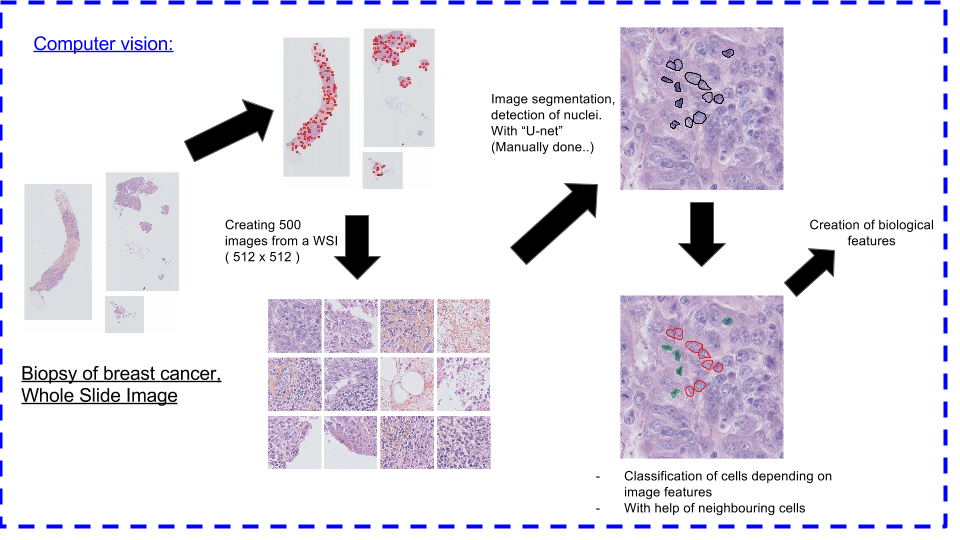
\includegraphics[width = 0.5\textwidth]{ComputerVision.png}

\section*{Uncovering information from histopathology data is a difficult task}

\begin{center}

  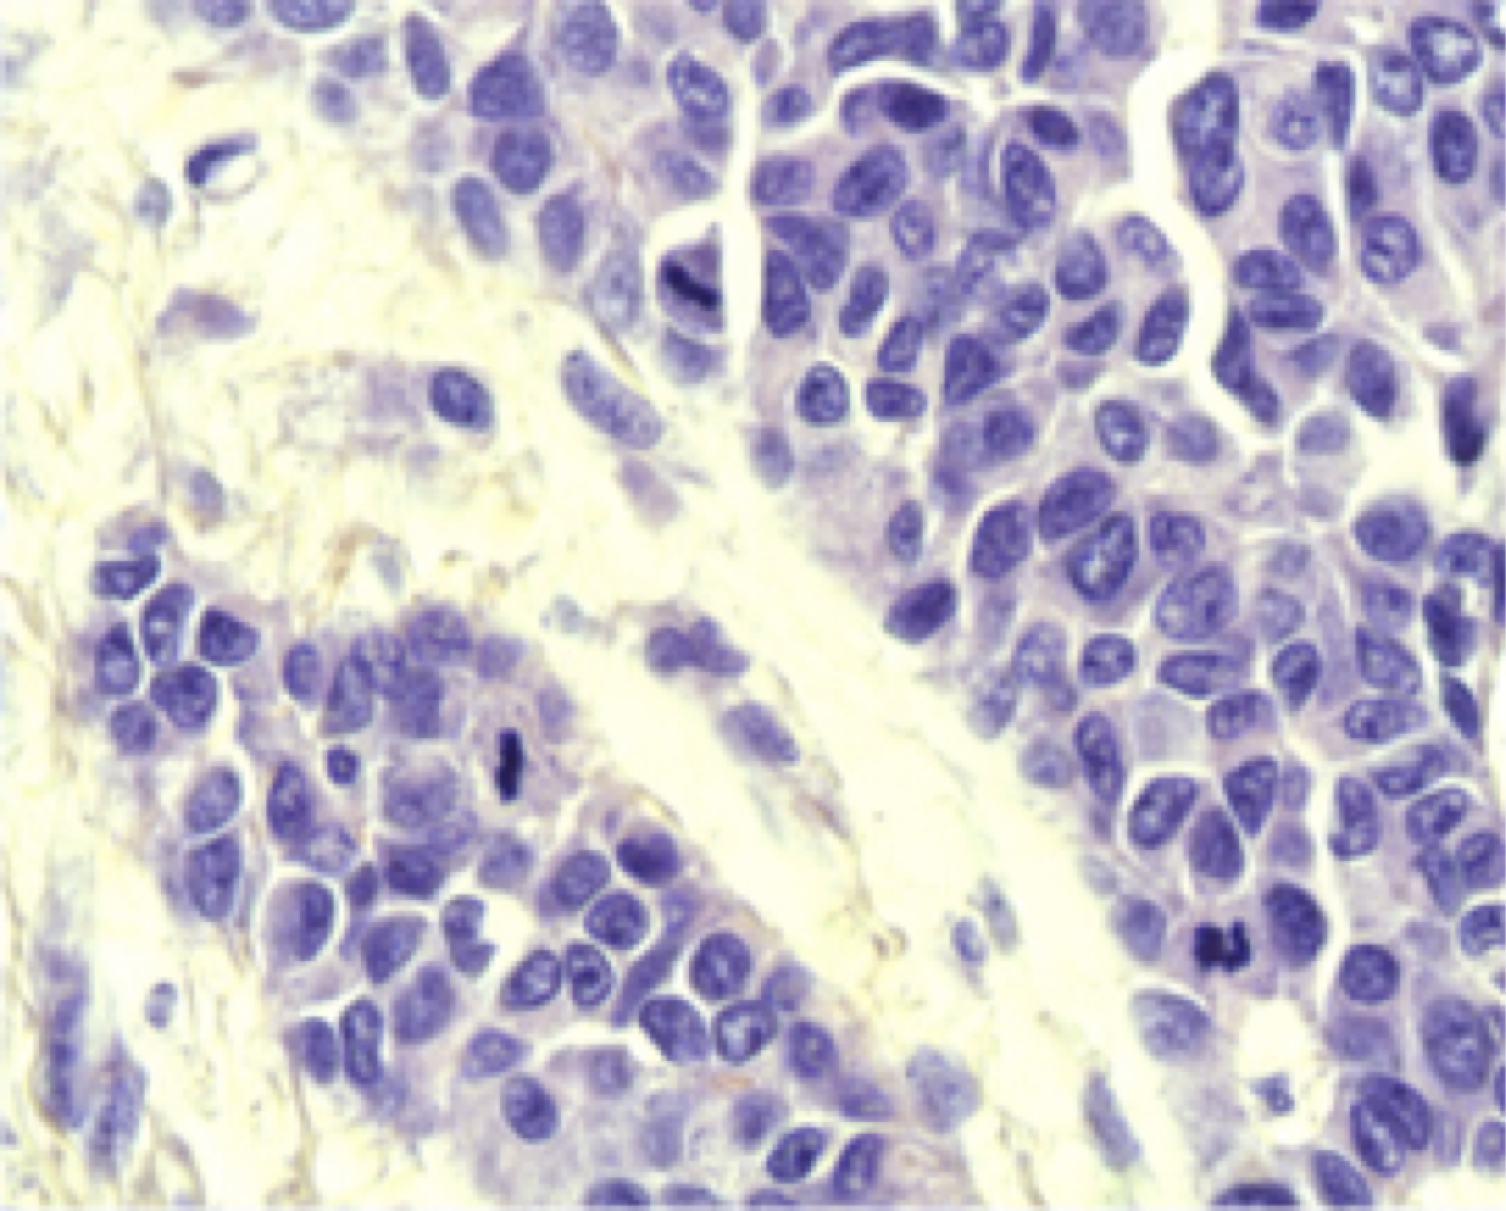
\includegraphics[height=12cm, width = 12cm]{histo1.png}
  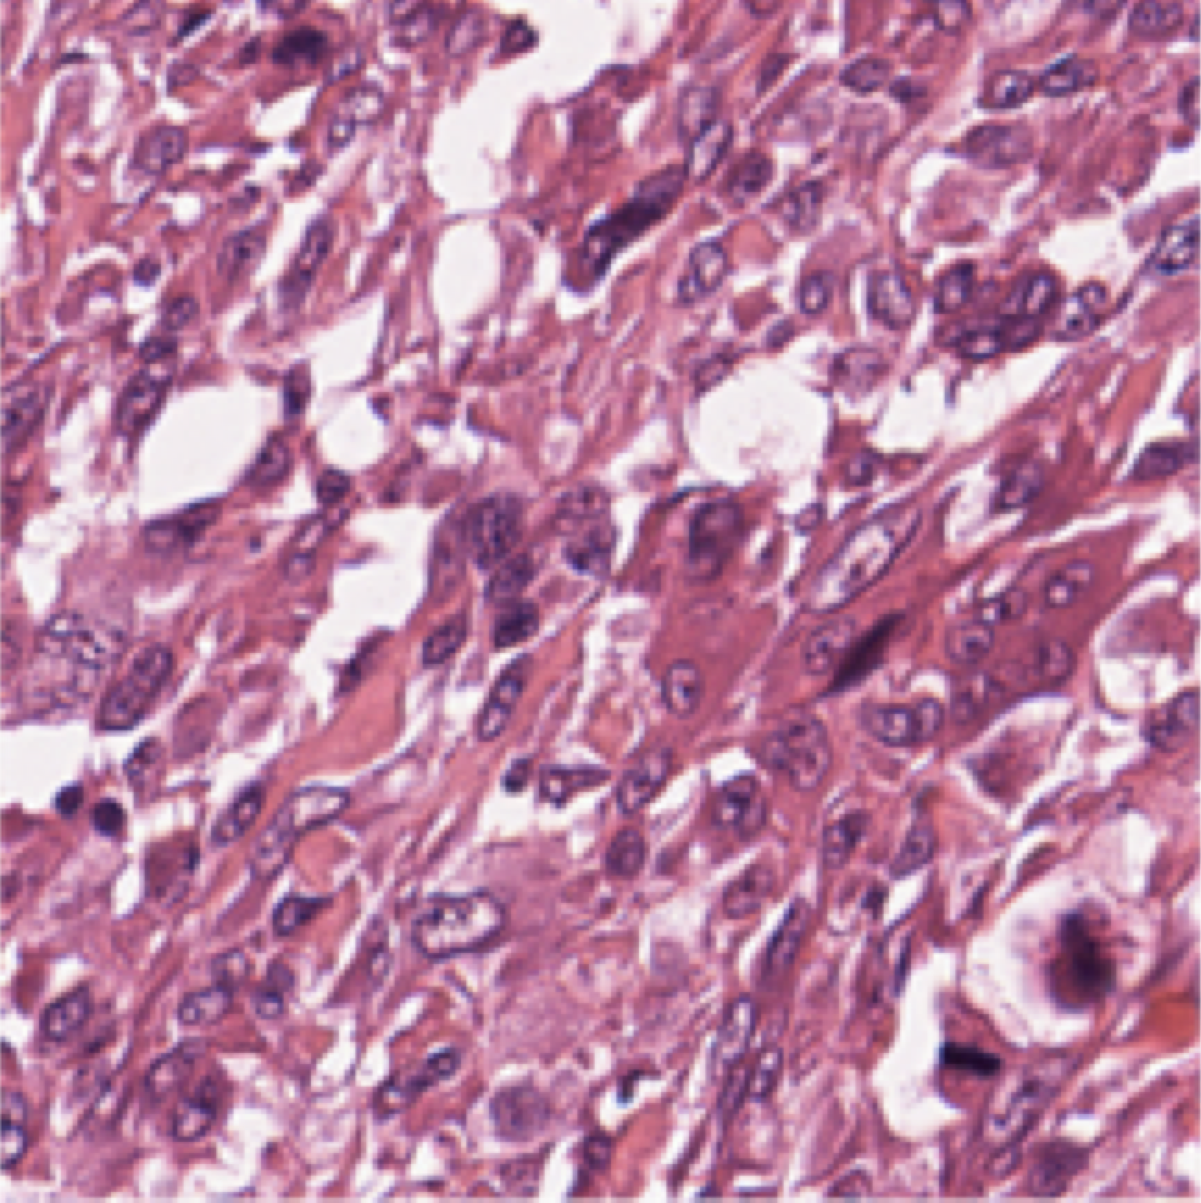
\includegraphics[height=12cm, width = 12cm]{histo2.png}
   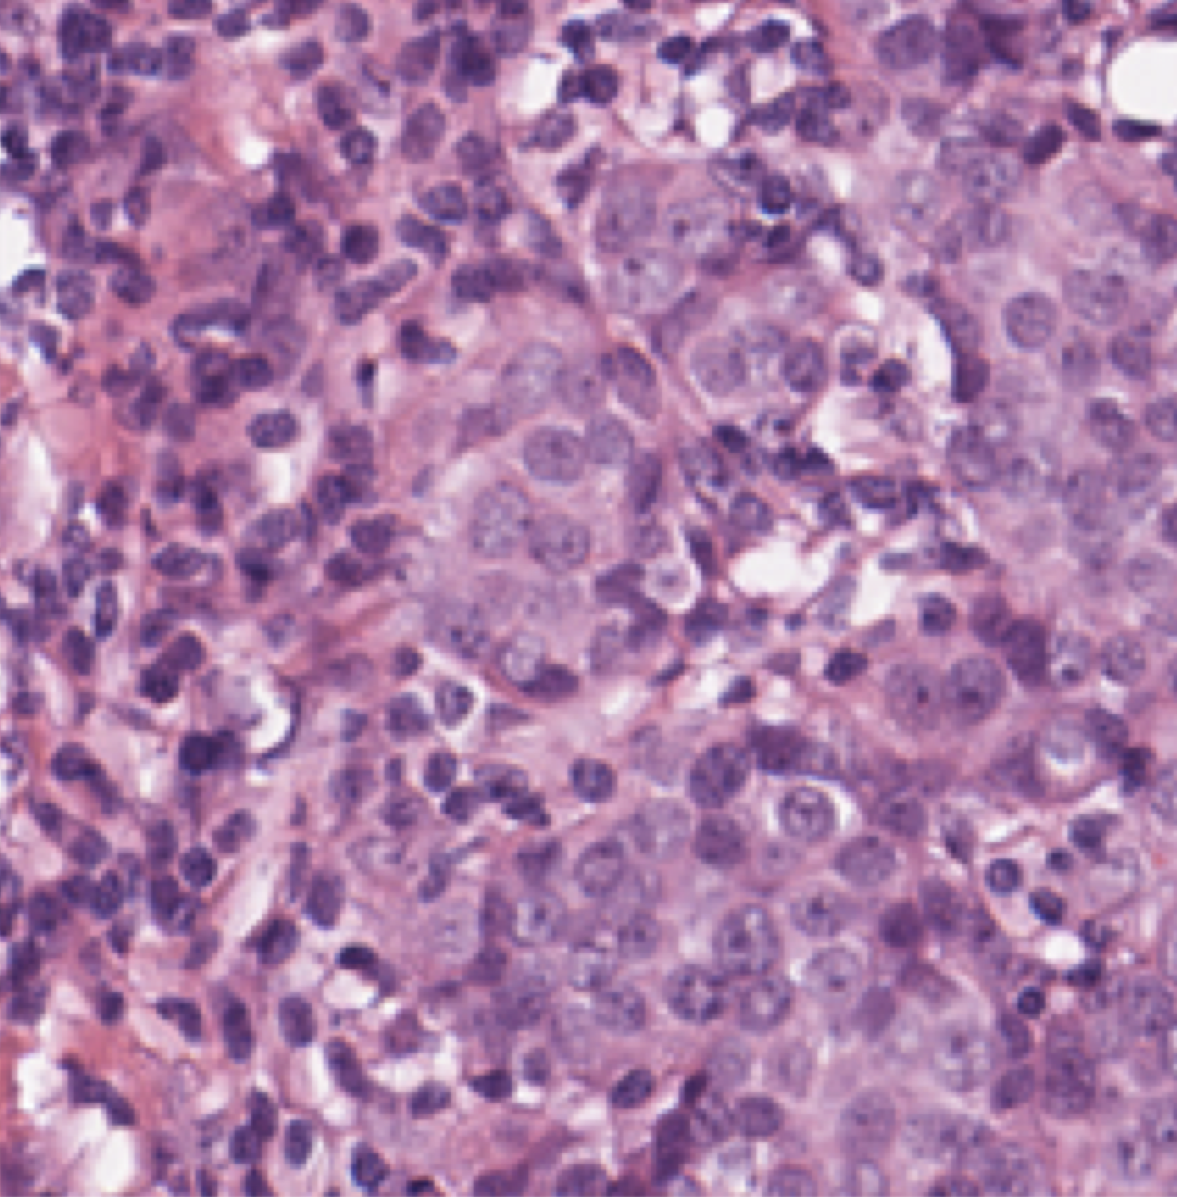
\includegraphics[height=12cm, width = 12cm]{histo3.png}
  \captionof{figure}{\color{Green} Histopathology data}
\end{center}

\begin{enumerate}
\item {\em Data size}: each patient has several slides, one slide is more than $50 GB$. A typical dataset: hundreds of slides. 

\item {\em Stain variation}: Many reasons for this variability : 
 scanner type, the stain supplier and
  the stain quality, differences in slide preparation and tissue
  type. 
\item {\em Variability in the objects}: another variability is biological variability. Many different cells and tissue types.
\item {\em Projection artefacts}: a slice is actually a 3D slice, we can have overlapping cells / nuclei
  and other artefacts.
\item {\em No explicit formalization of information}:
  No clear descriptions of the objects we are trying to identify.  
\end{enumerate}

\section*{Manual annotation of histopathology slides}

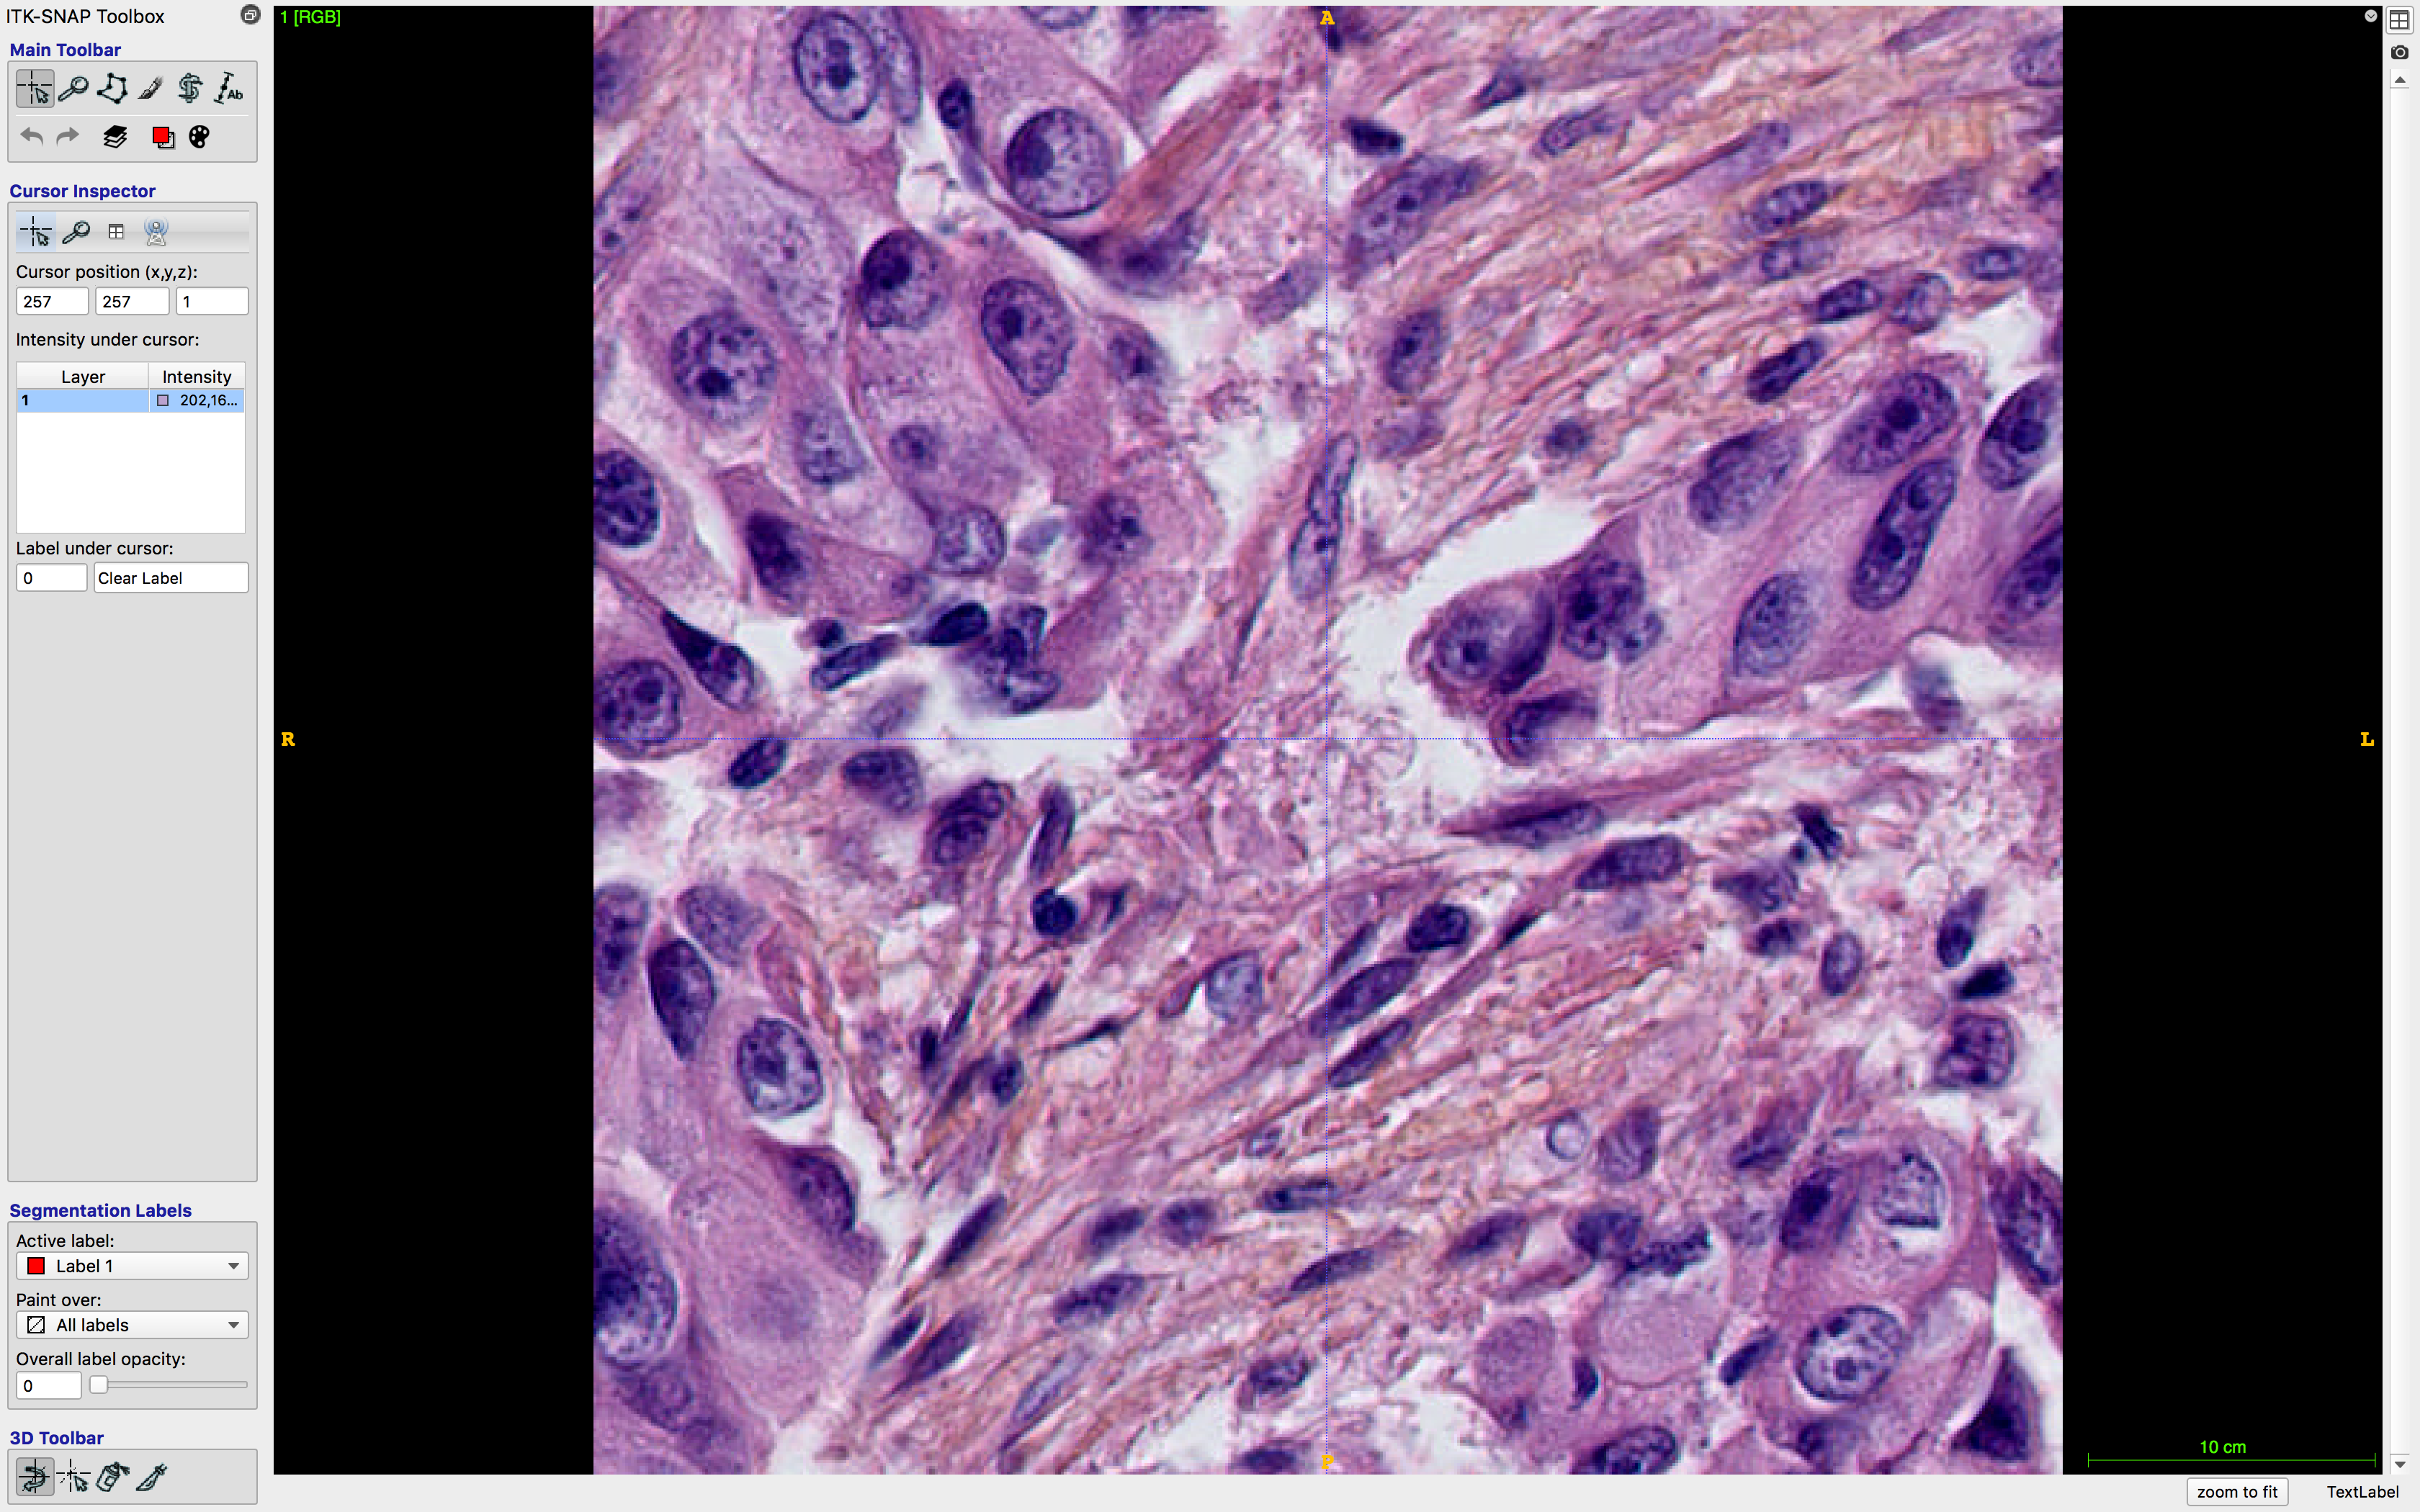
\includegraphics[height=10cm, width = 12cm]{Opacite0.png}
  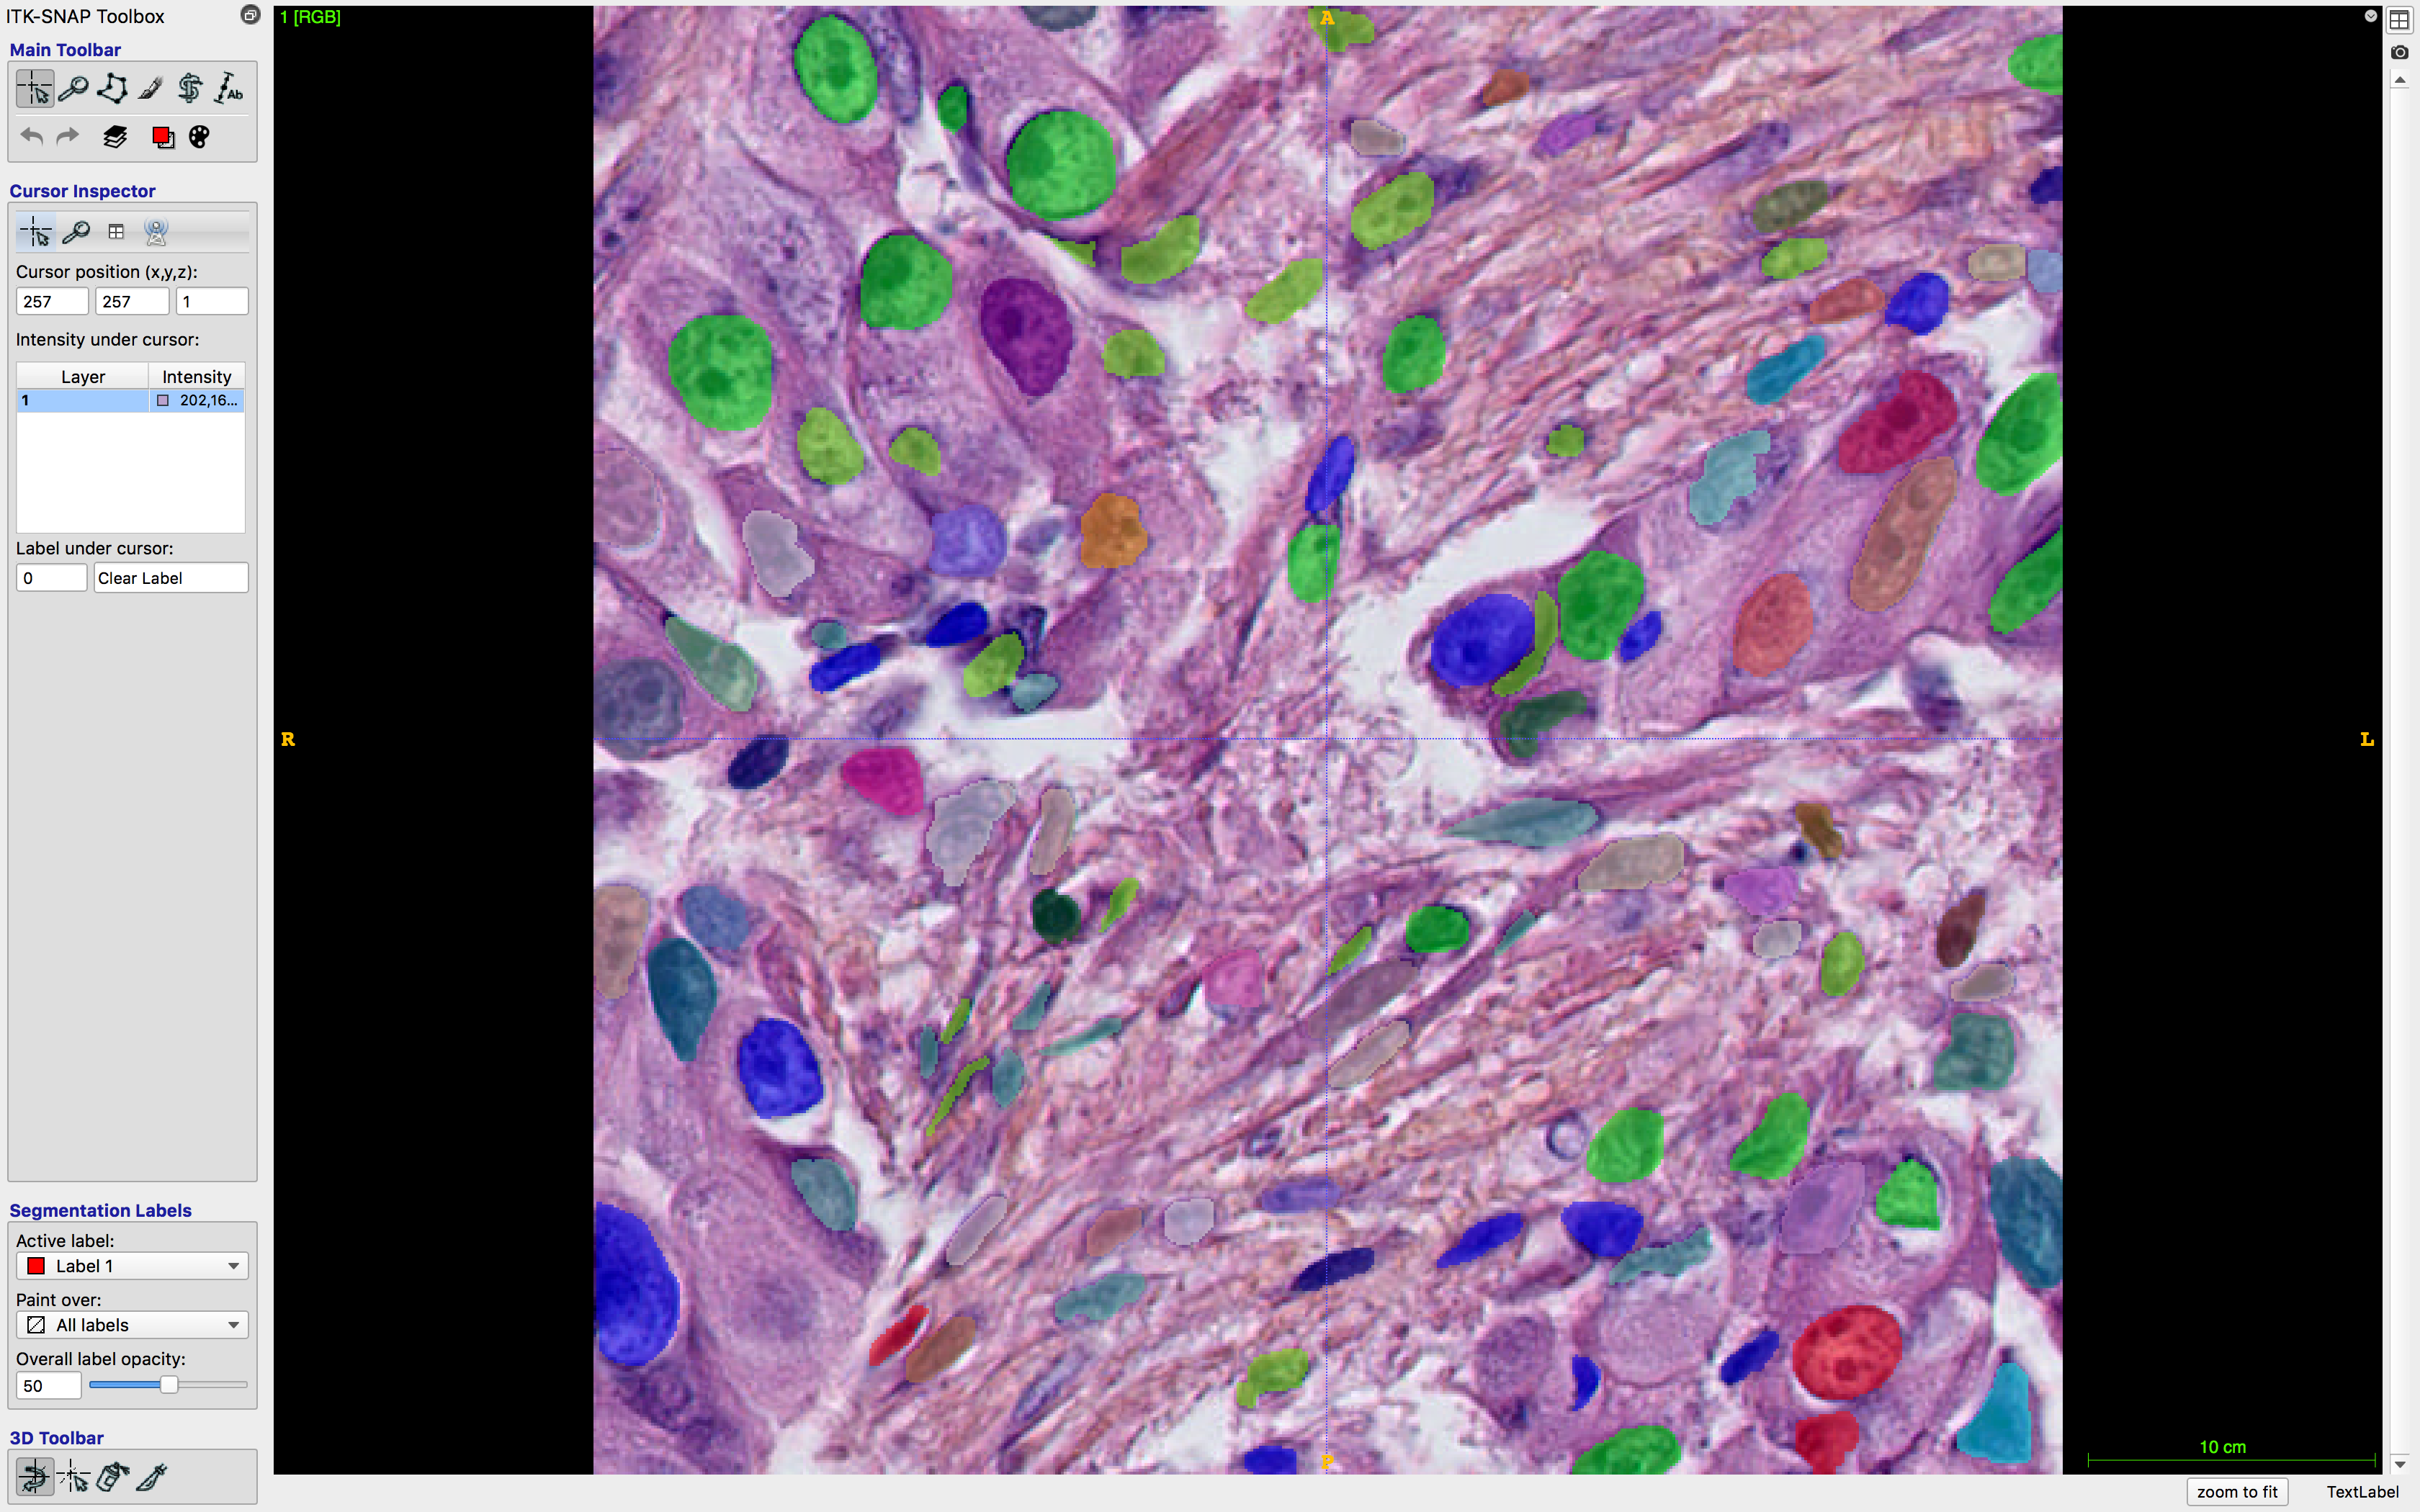
\includegraphics[height=10cm, width = 12cm]{Opacite50.png}
   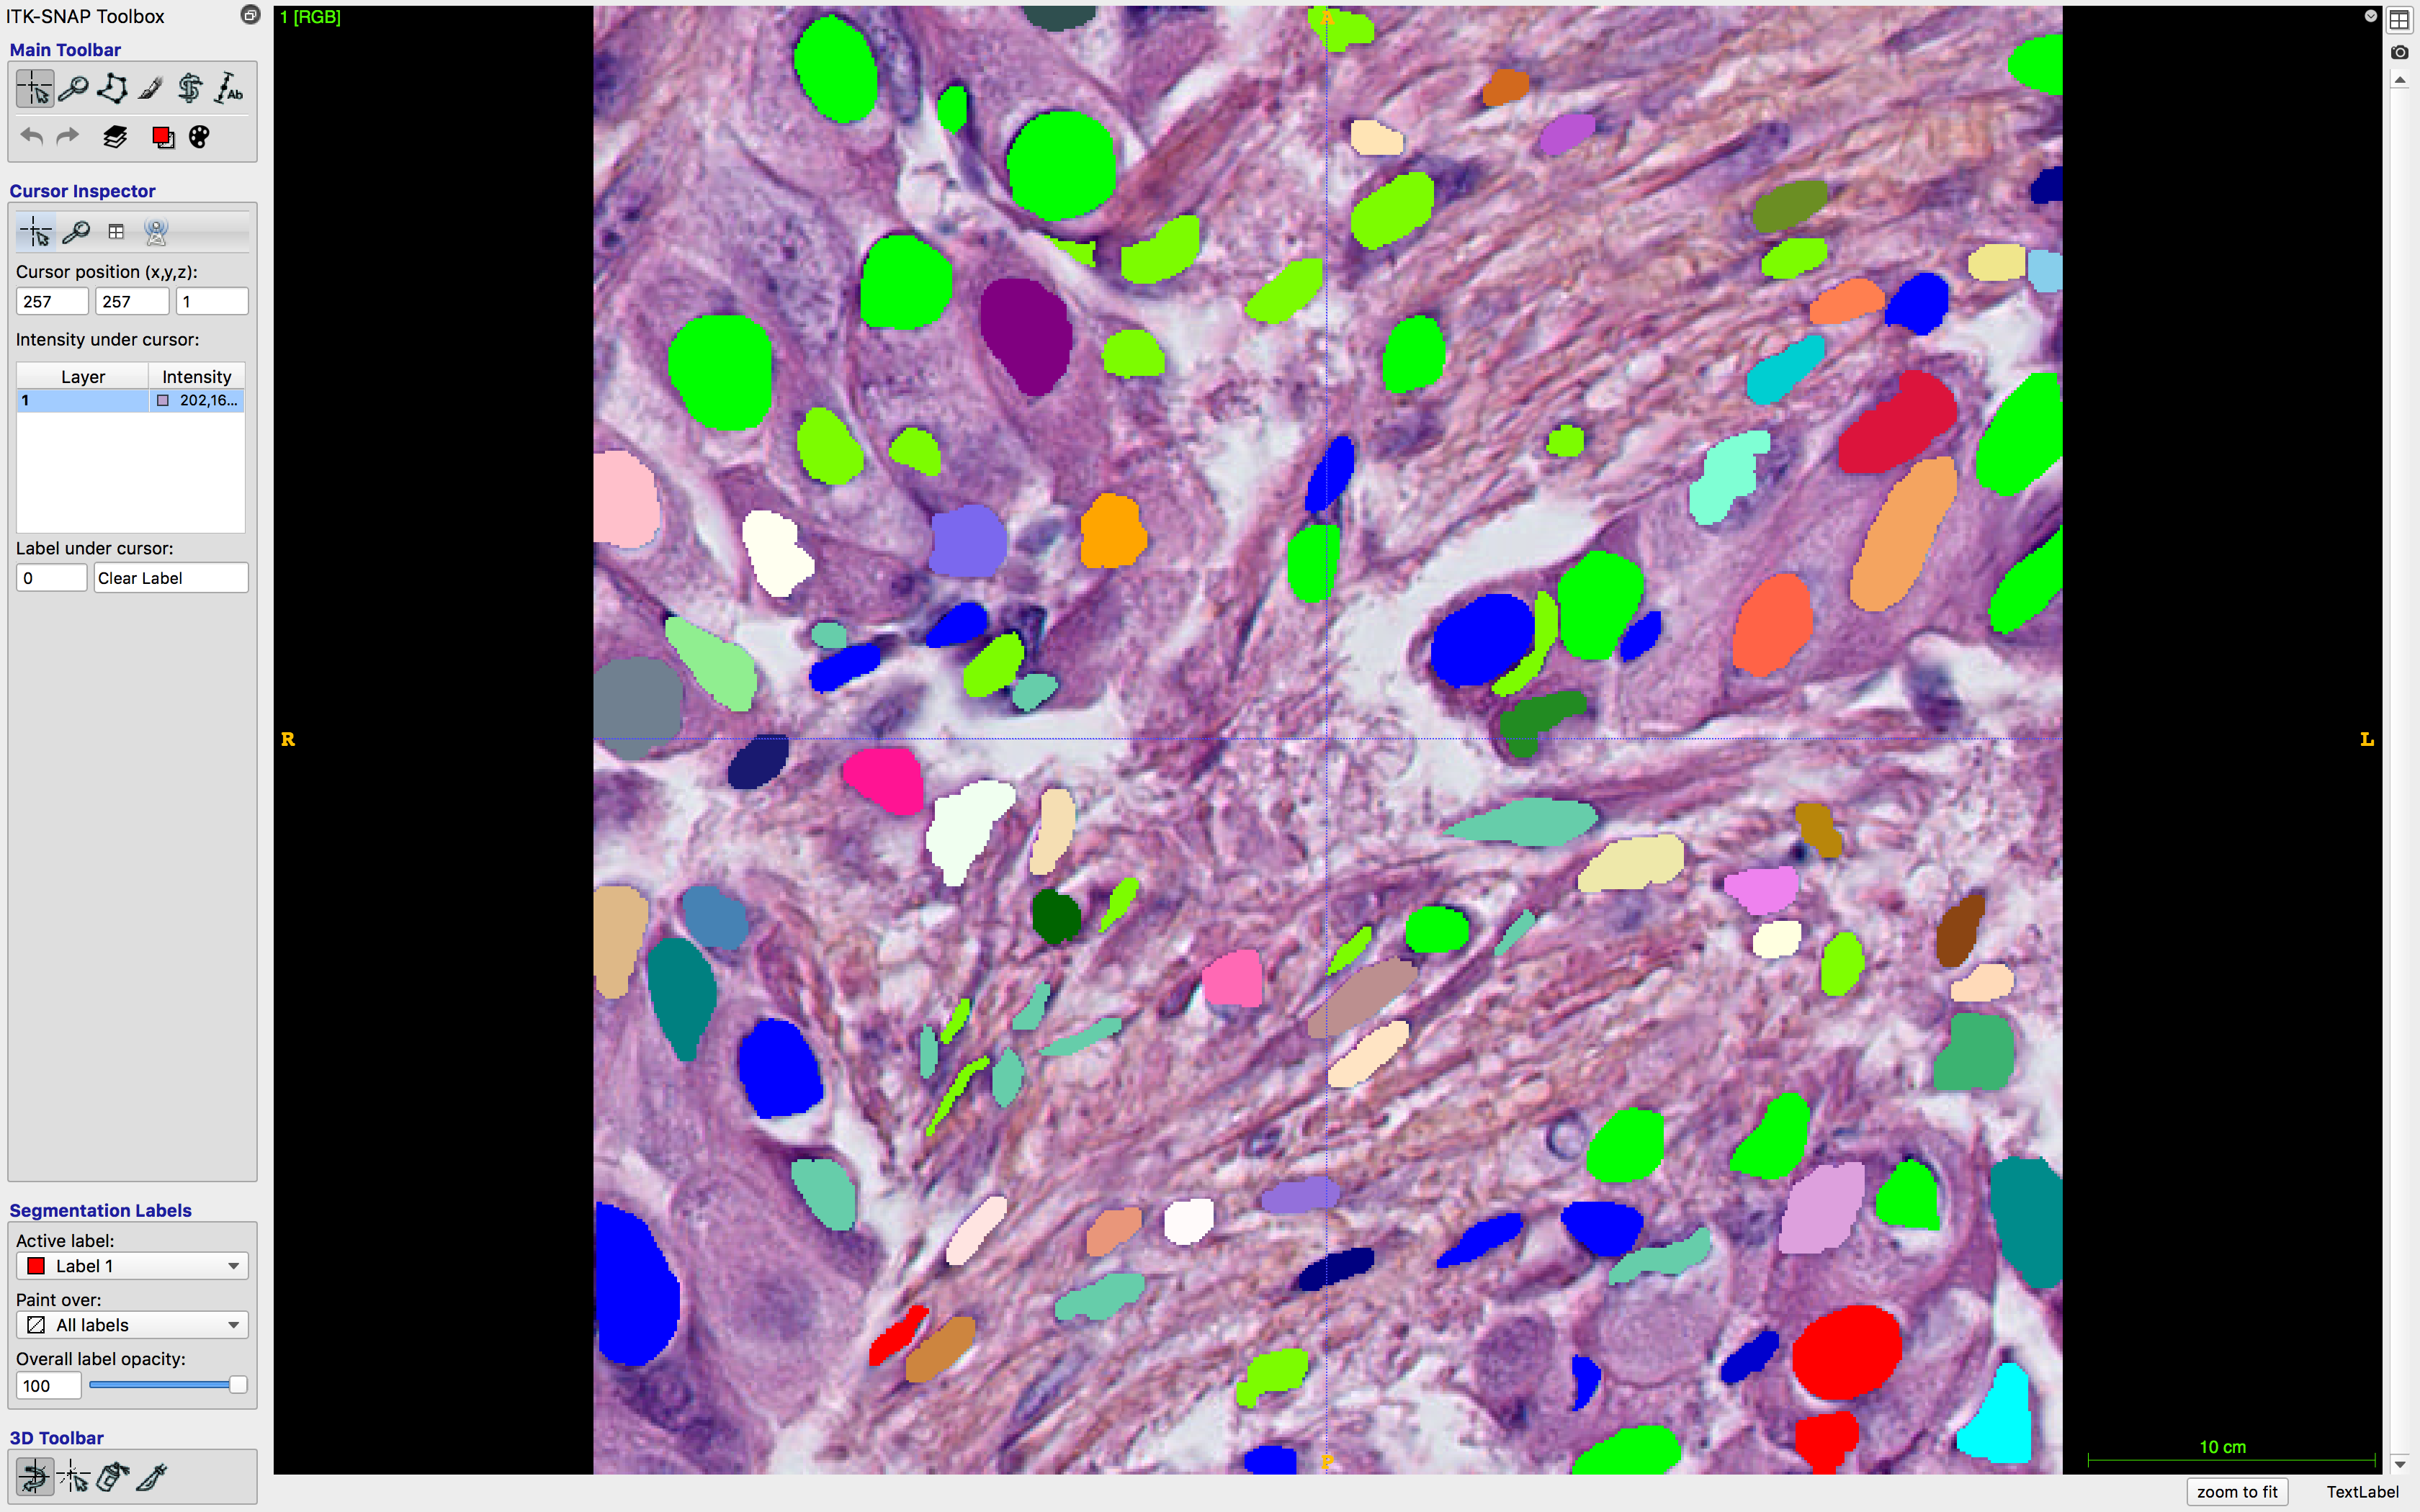
\includegraphics[height=10cm, width = 12cm]{Opacite100.png}
  \captionof{figure}{\color{Green} Histopathology data}

We use ITK-snap to manually annotate our histopathology slide. We wish to detect cells vs background. We have $33$ images of size $512 \times 512$ over $7$ different patients.

Cells can be very tricky to annotate: \\
\begin{multicols}{3}
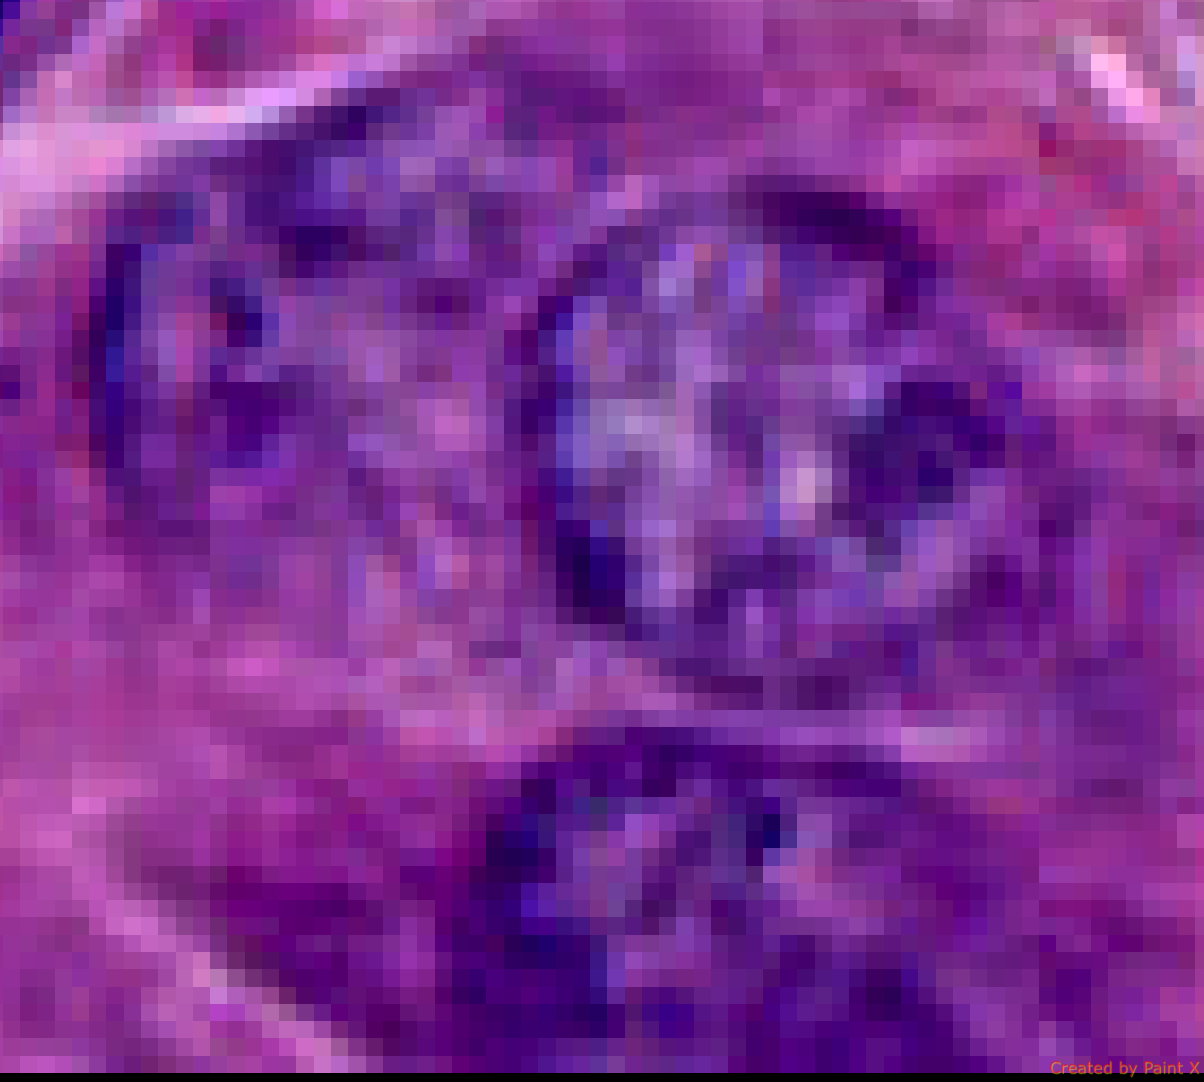
\includegraphics[height=5cm, width = 5cm]{under1.png}
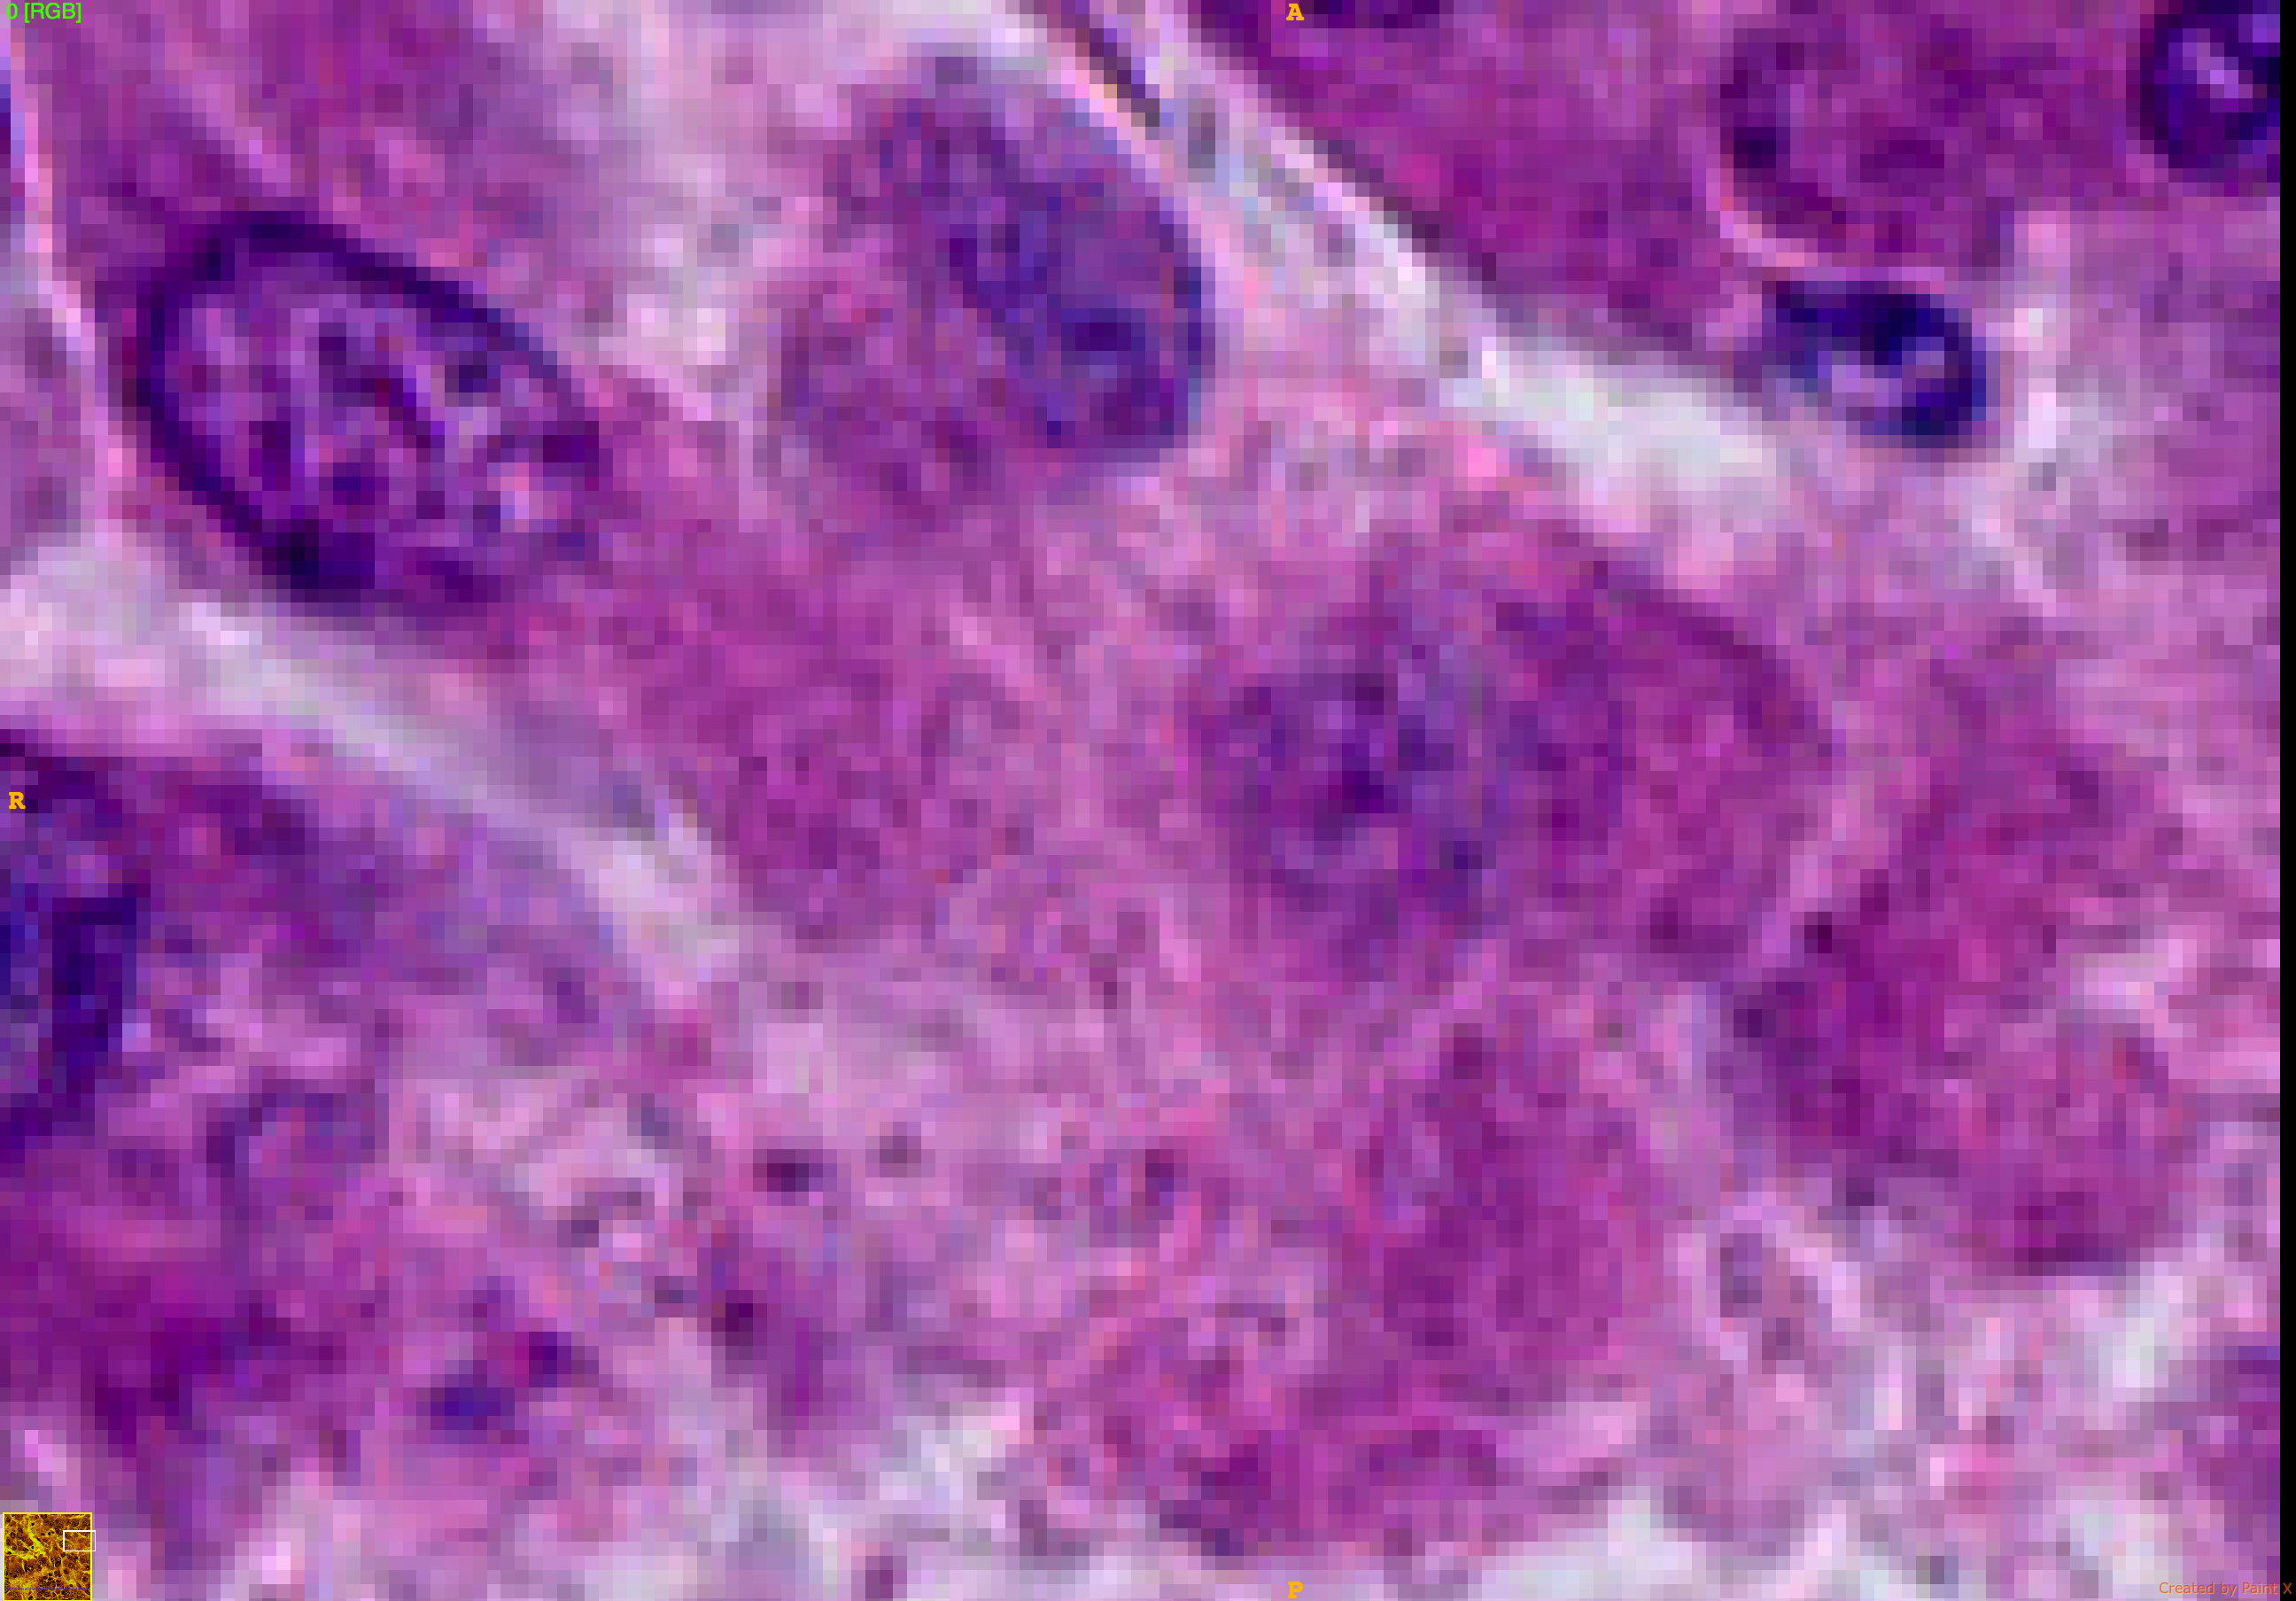
\includegraphics[height=5cm, width = 5cm]{under2.png}
\captionof{figure}{\color{Green} 3D Slice}
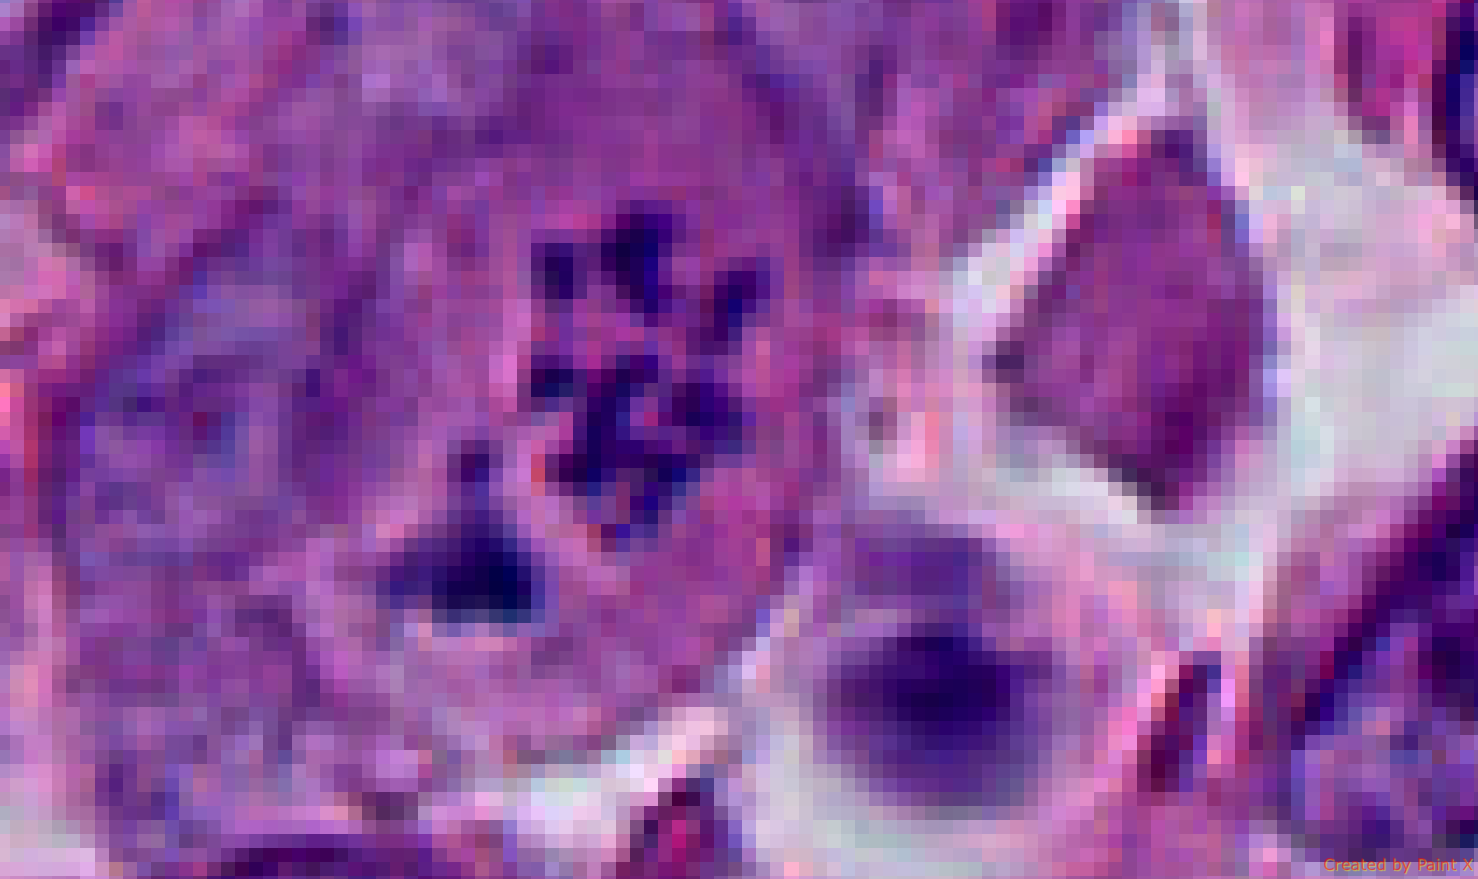
\includegraphics[height=5cm, width = 5cm]{mitose.png}
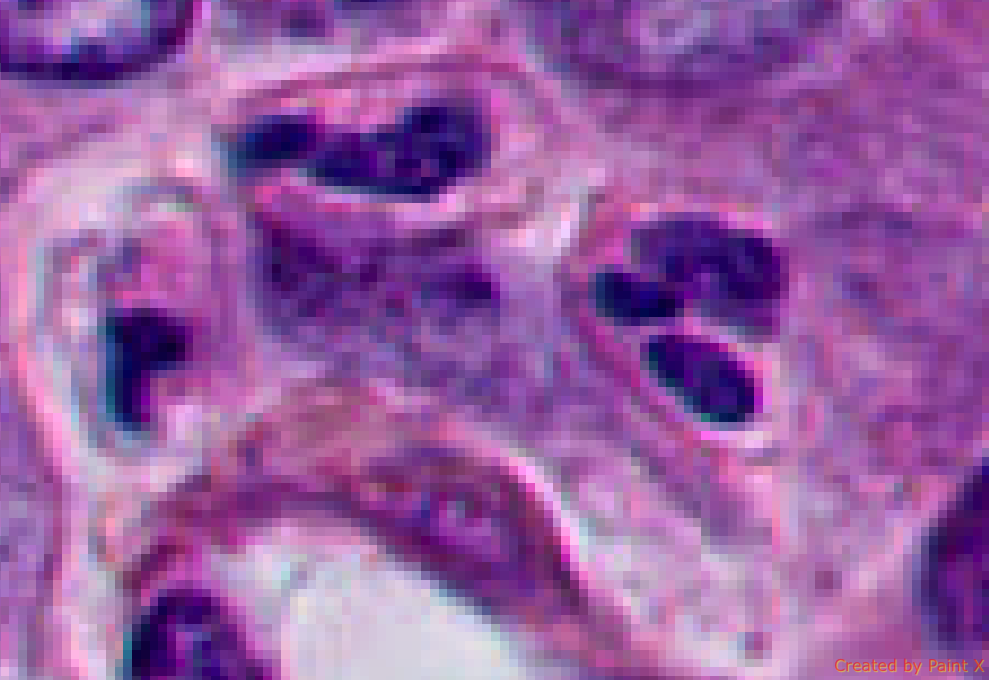
\includegraphics[height=5cm, width = 5cm]{mitose2.png}
\captionof{figure}{\color{Green} Wierd looking nuclei}
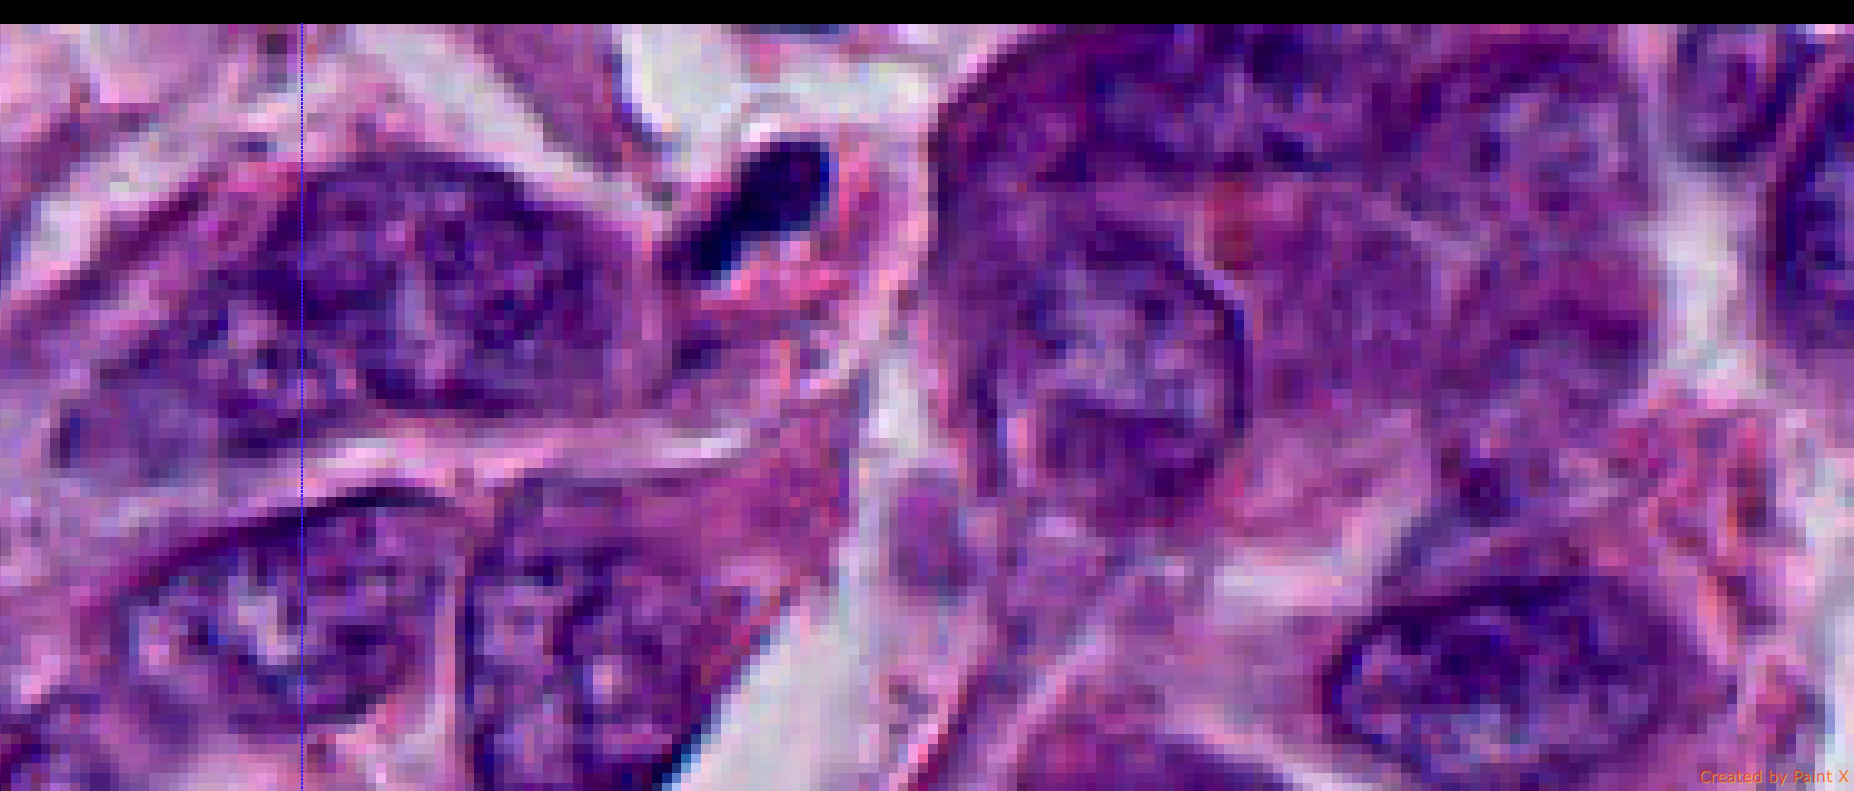
\includegraphics[height=5cm, width = 10cm]{clutered1.png}
\captionof{figure}{\color{Green} Dense region}
\end{multicols}
\section*{Fully Convolutionnal Networks (FCN)}
\begin{center}
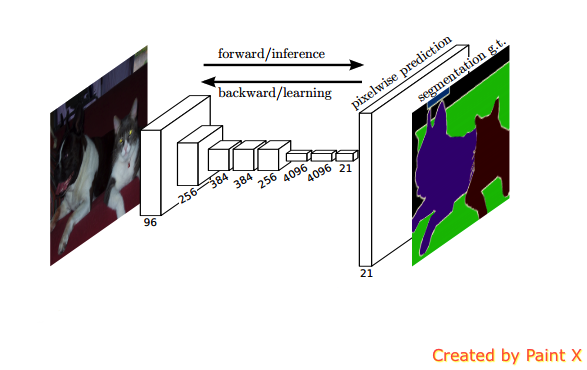
\includegraphics[trim={0 3cm 0 0},clip,width = 0.4\textwidth]{FCN.png}
\captionof{figure}{\color{Green} FCN for semantic segmentation (image taken from \cite{long2015fcn})}
\end{center}

FCN for segmentation are an extension of standard
 Convolutionnal network for image recognition. These models
 take an end to end tuned CNN, and cast it into a FCN.
  Upsampling and deconvolutionnal layers are added, the standard
 part of the CNN provides the "what" while the added layers try to provide the "where". 
Finally, skip path are added between layers to provide final layers 
with information from the first layers.

\section*{Results}

The fully convolutionnal network is fined tuned and helped with the use of data augmentation: rotation, flips, blurring and elastic deformation.
The size of the input images can be of $512\times512$ pixels or of 
 $256\times256$ pixels.  Several metrics were kept, especially: mean accuracy, intersection over union, the Jaccard Index, recall and precision.
Finally, training was performed on $21$ images and test on $5$ images across $6$ patients. $7$ validation images were used for reporting the validation scores, these validation images were provided by one patient.
\begin{center}
\begin{tabular}{l l l l l l}
\toprule
\textbf{Crop size} & \textbf{Network Name} & \textbf{MA} & \textbf{IU} & \textbf{Recall} & \textbf{Precision} \\
\midrule
512 & FCN8 & 0.54 & 0.52 & 0.09 & 0.12 \\
256 & FCN8 & 0.63 & 0.53 & 0.28 & 0.09 \\
256 & FCN8\_ 200 & 0.71 & 0.53 & 0.45 & 0.10 \\
256 & FCN8\_ 2000 & 0.65 & 0.53 & 0.31 & 0.11 \\
\bottomrule
\end{tabular}
\captionof{table}{\color{Green} First results}
\end{center}

%----------------------------------------------------------------------------------------
%	CONCLUSIONS
%----------------------------------------------------------------------------------------


%----------------------------------------------------------------------------------------
%	FORTHCOMING RESEARCH
%----------------------------------------------------------------------------------------

\section*{Forthcoming Research}

\color{SaddleBrown} % SaddleBrown color for the conclusions to make them stand out

\begin{itemize}
\item Setting up slighter different architectures: U-net \cite{UNet}.
\item Changing the loss to make it more adapted to segmentation, \cite{UNet}.
\item Changing the channels on the input, HE standardization \cite{deconvolution}.
\item Incorporating different prior knowledge about cell segmentation directly in the architecture. \cite{ranefall2016fast}.
\end{itemize}

\color{DarkSlateGray} % Set the color back to DarkSlateGray for the rest of the content

\bibliographystyle{plain}
%\bibliographystyle{abbrvnat}
\bibliography{biblio.bib} % Use the example bibliography file sample.bib


\end{multicols}
\end{document}